\chapter{水动力学问题差分解法}
\section{一维非恒定流求解}
\subsection{矩形明渠一维圣维南方程组}
对矩形断面渠道,一维圣维南方程组的守恒形式为:
\begin{equation}
  \frac{\partial \mathbf{U}}{\partial t} +
  \frac{\partial \mathbf{F}}{\partial x} =
  \mathbf{S}
\end{equation}
其中,$\mathbf{U}$为未知量矢量,$\mathbf{F}$为通量矢量,$\mathbf{S}$为源项矢量,
分别为:

\begin{equation}
  \mathbf{U} = 
  \begin{bmatrix}
    h \\
    v
  \end{bmatrix}
  ,
  \mathbf{F} = 
  \begin{bmatrix}
    hv \\
    hv^{2} + \frac{1}{2}gh^{2}
  \end{bmatrix}
  ,
  \mathbf{S} = 
  \begin{bmatrix}
    0 \\
    ghi - C_{f}v|v|
  \end{bmatrix}
\end{equation}
式中,$v(x,t)$为断面平均流速,$h(x,t)$为断面水深,$i$为底坡,$g$为重力加速度,
$C_{f}$为阻力系数。

\subsection{初始条件}
为了计算圣维南方程的瞬态解,必须要先知道所有网格节点上的水深和流速值。这些值不能
随意给定,而应该按照实际物理情况来给定初始条件,通常来说有两种选择。
\begin{enumerate}
  \item 渠道处于静止状态。在该状态下,水面为水平线,所有节点上的速度都为零。干燥区域也可以被包含在计算域中。
  \item 渠道处于恒定流状态。在该状态下,水深和流速必须通过恒定流水流求解手段来获得。这个求解过程主要是求解渐变流水面曲线方程来获得。如果渠道中存在急变流段,还需要求解水跃跃前跃后水深关系来获得。
    \begin{equation}
    \frac{\mathrm{d}h}{\mathrm{d}x}
    =
    \frac{i - J }{1 - Fr^{2 }}
    \end{equation}
    \begin{equation}
      \frac{h_{2 }}{h_{1 }}
      =
      \frac{1}{2 }
      [(1+8{Fr}_{1}^{2})^{1/2} - 1]
    \end{equation}
\end{enumerate}

\subsection{边界条件}

\subsection{显式格式}

\subsubsection{FTCS格式}
时间用一阶向前差分,空间上用二阶中心差分格式的FTCS格式可能是最简单的差分格式。可
是,这一格式是不稳定的,因而这一格式也就被称为不稳定格式。
\begin{equation}
  \mathbf{U}_{i}^{k+1} 
  =
  \mathbf{U}_{i}^{k} -
  \frac{\Delta t}{2\Delta x}(\mathbf{F}_{i+1}^{k}-\mathbf{F}_{i}^{k}) + 
  \mathbf{S}_{i}^{k}\Delta t
\end{equation}
通过设定极低的CFL值,外加引入人工粘性来抑制振荡,该格式可用。然而,这格式没有使
用价值。

\subsubsection{Lax扩散格式}
Lax扩散格式是非稳定格式的一个变体,是一个具有激波捕捉能力的单步差分格式,却在数
值上扩散。该格式如下:
\begin{equation}
  \mathbf{U}_{i}^{k+1} 
  =
  \frac{(\mathbf{U}_{i-1}^{k} + \mathbf{U}_{i+1}^{k})}{2} -
  \frac{\Delta t}{2\Delta x}(\mathbf{F}_{i+1}^{k}-\mathbf{F}_{i}^{k}) + 
  \mathbf{S}_{i}^{k}\Delta t
\end{equation}
采用泰勒级数将上式中各项在$k$时间层和节点$i$上展开,当$\Delta x$和$\Delta
t\rightarrow 0$时,上式变为
\begin{equation}
  \frac{\partial \mathbf{U}}{\partial t} +
  \frac{\partial \mathbf{F}}{\partial t} =
  \frac{1}{2}D\frac{{\partial}^{2} \mathbf{U}}{\partial {x}^{2}} +
  \mathbf{S}
\end{equation}
其中,$D$是计算网格上类似的扩散系数,
\begin{equation}
D =
\frac{(\Delta x)^{2}}{\Delta t}
\end{equation}
由此可见,Lax扩散格式是不相容的。因此,对给定的$\Delta x$,如果降低CFL值,计算采
用的$\Delta t$也会降低,$D$会增加,求解过程中会表现出更大的扩散性。因此,该扩散
格式具有网格相关性。


%\subsubsection{迎风格式}

\subsubsection{MacCormack预测校正格式}
MacCormack格式是一种两步(预测步和校正步)有限差分格式,具备激波捕捉能力。在预测
步,通量$\mathbf{F}$采用向前差分格式,用$k$时间层信息来计算。
\begin{equation}
  \mathbf{U}^{\mathrm{yc}} =
  \mathbf{U}^{k} -
  \frac{\Delta t }{\Delta x }
  (\mathbf{F}_{i}^{k} - \mathbf{F}_{i}^{k}) +
  \mathbf{S}_{i}^{k}\Delta t
\end{equation}
预测步给出了$k+1$时间层的流动的近似值,记为预测值。在校正步,通量$\mathbf{F}$采
用向后差分格式,用$k+1$时间层信息来计算。
\begin{equation}
  \mathbf{U}^{\mathrm{jz}} =
  \mathbf{U}^{k} -
  \frac{\Delta t }{\Delta x }
  (\mathbf{F}_{i}^{\mathrm{yc}} - \mathbf{F}_{i}^{\mathrm{yc}}) +
  \mathbf{S}_{i}^{\mathrm{yc}}\Delta t
\end{equation}
$k+1$时间层的最终结果是预测步和校正步得出的结果取平均得到的。
\begin{equation}
  \mathbf{U}^{k+1} =
  \mathbf{U}^{\mathrm{pj}} =
  \frac{1}{2}
  (\mathbf{U}^{\mathrm{yc}} +\mathbf{U}^{\mathrm{jz}})
\end{equation}

MacCormack格式在时间和空间上都是二阶精度,也是条件稳定的,因此受到CFL条件的限制。
根据Godunov理论,精度高于一阶的格式将在$\mathbf{U}$梯度较高的区域内产生非物理振
荡,比如在激波附近,例如溃坝波的波头。一阶精度格式虽然不会引入非物理振荡,但是过
度的扩散抹平了波头。因此,在实际使用中,二阶格式常被采用,控制非物理振荡的策略是
在局部区域内根据需要引入一定量的数值扩散。

\subsubsection{带人工粘性的MacCormack格式}
MacCormack格式中非物理振荡可以通过引入人工扩散来降低。在预测和校正步后,人工粘性
的引入是通过求解下面的附加方程
\begin{equation}
  \frac{\partial \mathbf{U}}{\partial t} =
  \varepsilon
  \frac{(\Delta x)^{2}}{\Delta t}
  \frac{{\partial}^{2}\mathbf{U}}{\partial x^{2}}
\end{equation}
式中,$\varepsilon$是一个扩散系数,用来控制格式中的耗散量。当$\varepsilon$取常数
时,上式中扩散项用二阶中心格式离散,可得
\begin{equation}
  \mathbf{U}_{i}^{k+1} =
  \mathbf{U}_{i}^{\mathrm{pj}} +
  \varepsilon
  (
  \mathbf{U}_{i+1}^{\mathrm{pj}} - 
  2\mathbf{U}_{i}^{\mathrm{pj}} +
  \mathbf{U}_{i-1}^{\mathrm{pj}}
  )
\end{equation}
基于这一思想,Jameson等人\cite{ref6}提出一种更容易实现的方法。上式改写为:
\begin{equation}
  \mathbf{U}_{i}^{k+1} =
  \mathbf{U}_{i}^{\mathrm{pj}} +
  {\varepsilon}_{i+1/2}
  (
  \mathbf{U}_{i+1}^{\mathrm{pj}} - 
  \mathbf{U}_{i}^{\mathrm{pj}}
  )
  -
  {\varepsilon}_{i-1/2}
  (
  \mathbf{U}_{i}^{\mathrm{pj}} -
  \mathbf{U}_{i-1}^{\mathrm{pj}}
  )
\end{equation}
其中,
\begin{equation}
  {\varepsilon}_{i+1/2} =
  K\max({\varepsilon}_{i+1}-{\varepsilon}_{i})
\end{equation}
${\varepsilon}_{i}$是基于水深计算得出的参数。
\begin{equation}
  {\varepsilon}_{i} =
  \frac{|h_{i+1}-2h_{i}+h_{i-1}|}{|h_{i+1}|+2|h_{i}|+|h_{i-1}|}
\end{equation}
$K$为人工粘性系数,需要校验,通常取值范围为0.5\textasciitilde 3。这一格式只在振荡发展区域内引入
数值扩散,而其他区域内的解不受影响。

\subsubsection{TVD MacCormack格式}
总变分减少(total variation diminishing, TVD)格式是高阶格式,可得到更加尖锐的激
波解,并引入对解的界来避免出现虚假的振荡。一个函数$f$的总变分(TV)可定义为,
\begin{equation}
  TV(f) =
  \sum_{i=-\infty}^{\infty}
  |{f}_{i+1} - {f}_{i}|
\end{equation}
当差分格式满足下式时,该格式就是TVD的。
\begin{equation}
  TV({f}^{k+1}) \le TV({f}^{k})
\end{equation}
TVD格式在光滑解区域是二阶精度的,在非连续区域附近侦测到高梯度出现时
降低到一阶精度,以便压制虚假振荡。
二阶精度引入的数值弥散可通过在必要时引入数值扩散,切换到一阶精度格式,来抑制。

MacCormack格式的TVD格式由Garcia-Navarro\cite{ref7}等于1992年给出。在预测和校正步后,最终解
通过增加一个耗散项来得出,
\begin{equation}
  \mathbf{U}_{i}^{k+1} =
  \mathbf{U}_{i}^{pj} +
  \frac{\Delta t}{\Delta x}
  \left(
    \mathbf{D}_{i+1/2}^{k} -
    \mathbf{D}_{i-1/2}^{k}
  \right)
\end{equation}
式中,扩散项$\mathbf{D}_{i+1/2}$由下式给出
\begin{equation}
  \mathbf{D}_{i+1/2}^{k} =
  \frac{1}{2}
  \sum_{n=1}^{2}
  \alpha_{i+1/2}^{n}
  \psi_{i+1/2}^{n}
  \left(
    1 - 
    \frac{\Delta t}{\Delta x}
    \left|
    \lambda_{i+1/2}^{n}
    \right|
  \right)
  \left(
    1-\phi_{i+1/2}^{n}
  \right)
  \mathbf{e}_{i+1/2}^{n}
\end{equation}
平均速度和波速如下
\begin{equation}
  v_{i+1/2} = 
  \frac
  {v_{i}\sqrt{h_{i}} + v_{i+1}\sqrt{h_{i+1}}}
  {\sqrt{h_{i}}+\sqrt{h_{i+1}}}
  ,\quad
  c_{i+1/2} =
  \left(
    g 
    \frac{h_{i}+h_{i+1}}{2}
  \right)^{1/2}
\end{equation}
特征值和平均特征值如下
\begin{equation}
  \lambda_{i}^{1,2} = v_{i}\pm c_{i}
  ,\quad
  \lambda_{i+1/2}^{1,2} = v_{i+1/2}\pm c_{i+1/2}
\end{equation}
特征向量定义如下
\begin{equation}
  \mathbf{e}_{i+1/2}^{1,2} 
  =
  \begin{bmatrix}
    1 \\
    \lambda_{i+1/2}^{1,2}
  \end{bmatrix}
\end{equation}
函数$\psi$是一个定熵函数,用来避免非物理跳跃,由下式给出
\begin{equation}
  \psi_{i+1/2}^{1,2} =
  \begin{cases}
    |\lambda_{i+1/2}^{1,2}| & \mathrm{if} \quad |\lambda_{i+1/2}^{1,2}| \ge \varepsilon_{i+1/2}^{1,2} \\
    \varepsilon_{i+1/2}^{1,2} & \mathrm{else}
  \end{cases}
\end{equation}
其中,
\begin{equation}
\varepsilon_{i+1/2}^{1,2} =
\max 
\left(
  0,
  \lambda_{i+1/2}^{1,2} - \lambda_{i}^{1,2},
  \lambda_{i+1}^{1,2} - \lambda_{i+1/2}^{1,2}
\right)
\end{equation}
在节点$i$和$i+1$之间的$\mathbf{U}$在特征向量$\mathbf{e}_{i+1/2}^{1,2}$上的投影为
\begin{equation}
\alpha_{i+1/2}^{1,2} = 
\frac{1}{2c_{i+1/2}^{1}}
\left[
  \mp\lambda_{i+1/2}^{2,1}(h_{i+1}-h_{i})
  \pm
  (q_{i+1} - q_{i})
\right]
\end{equation}
函数$\phi$是一个通量限制器,可采用下式计算。
\begin{equation}
\phi_{i+1/2}^{1,2} =
\frac{r_{i+1/2}^{1,2}+(r_{i+1/2}^{1,2})^{2}}{1+(r_{i+1/2}^{1,2})^{2}}
\end{equation}
其中,
\begin{equation}
r_{i+1/2}^{1,2} =
\frac{\alpha_{i+1/2-s}^{1,2}}{\alpha_{i+1/2}^{1,2}}
\end{equation}
\begin{equation}
s = 
\mathrm{sign}
\left(
  \lambda_{i+1/2}^{1,2}
\right)
\end{equation}
该格式无需调参,且易于实现,推荐使用。

% ToDo List start
%\subsubsection{迎风格式}

%\subsection{隐式格式}
%\subsubsection{FTCN格式}
%\subsubsection{龙格库塔CN格式}
%\subsubsection{Pressimann格式}

% ToDo List end
\subsection{下游有水的缓流溃坝波}
考虑光滑平底矩形渠道内的溃坝波问题。
渠道总长$L=100\mathrm{m}$,
坝面所在位置$x=30\mathrm{m}$,
上游水深$h_{u}=0.2\mathrm{m}$,
下游水深$h_{d}=0.1\mathrm{m}$。
三种MacCormack格式计算结果如图\ref{FgEx_ori_result_t_5}、\ref{FgEx_art_result_t_5}和\ref{FgEx_tvd_result_t_5}所示。
\begin{figure}[!htb]
  \centering
  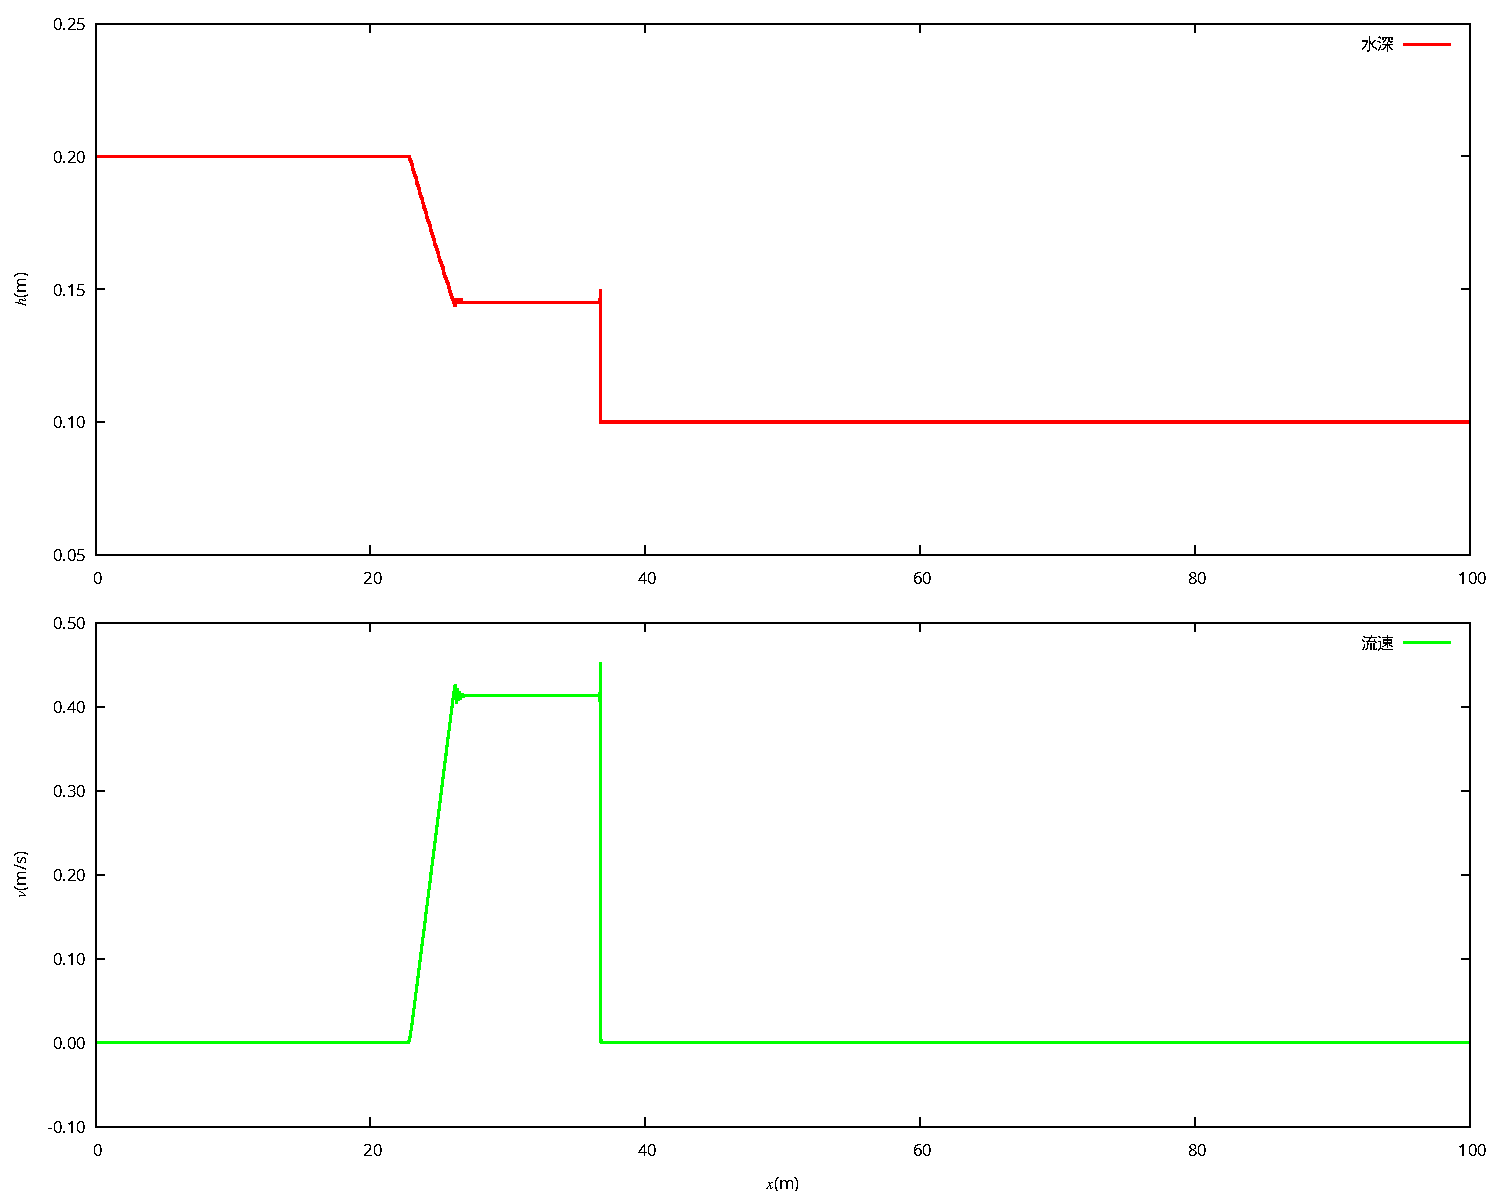
\includegraphics[width=8cm]{FgEx_ori_result_t_5.pdf}
  \caption{MacCormack格式计算结果}
  \label{FgEx_ori_result_t_5}
\end{figure}
\begin{figure}[!htb]
  \centering
  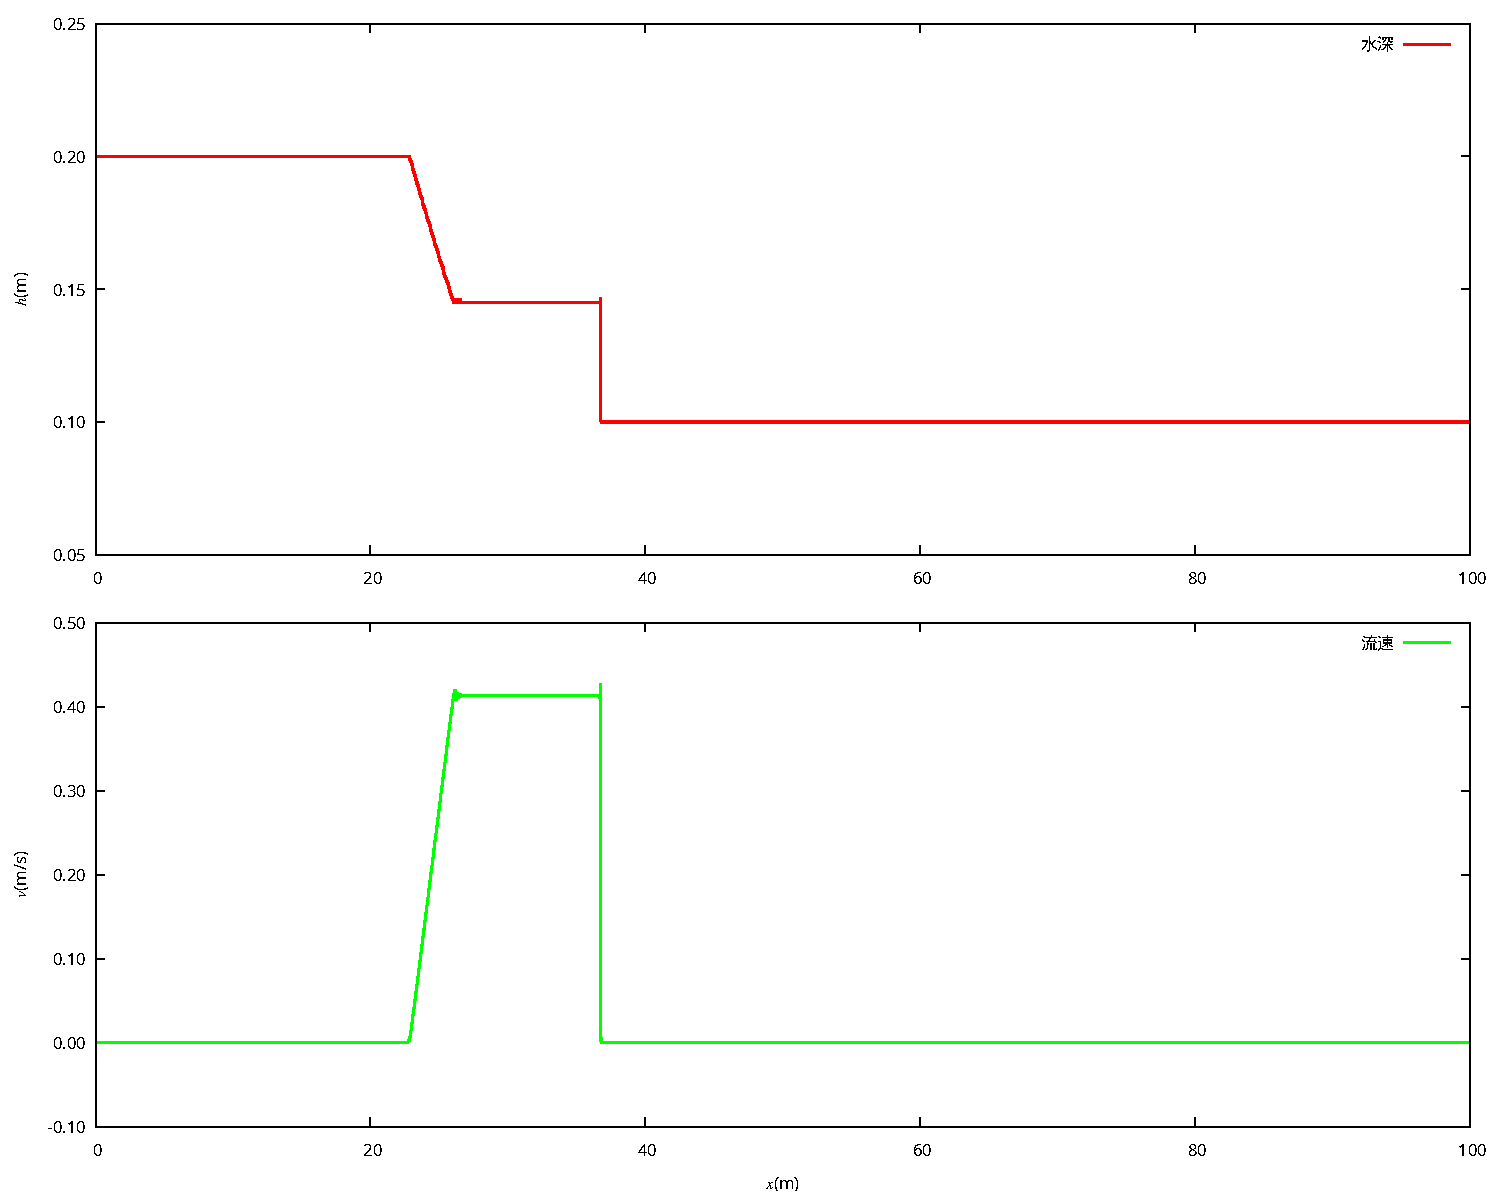
\includegraphics[width=8cm]{FgEx_art_result_t_5.pdf}
  \caption{MacCormack人工粘性格式计算结果}
  \label{FgEx_art_result_t_5}
\end{figure}
\begin{figure}[!htb]
  \centering
  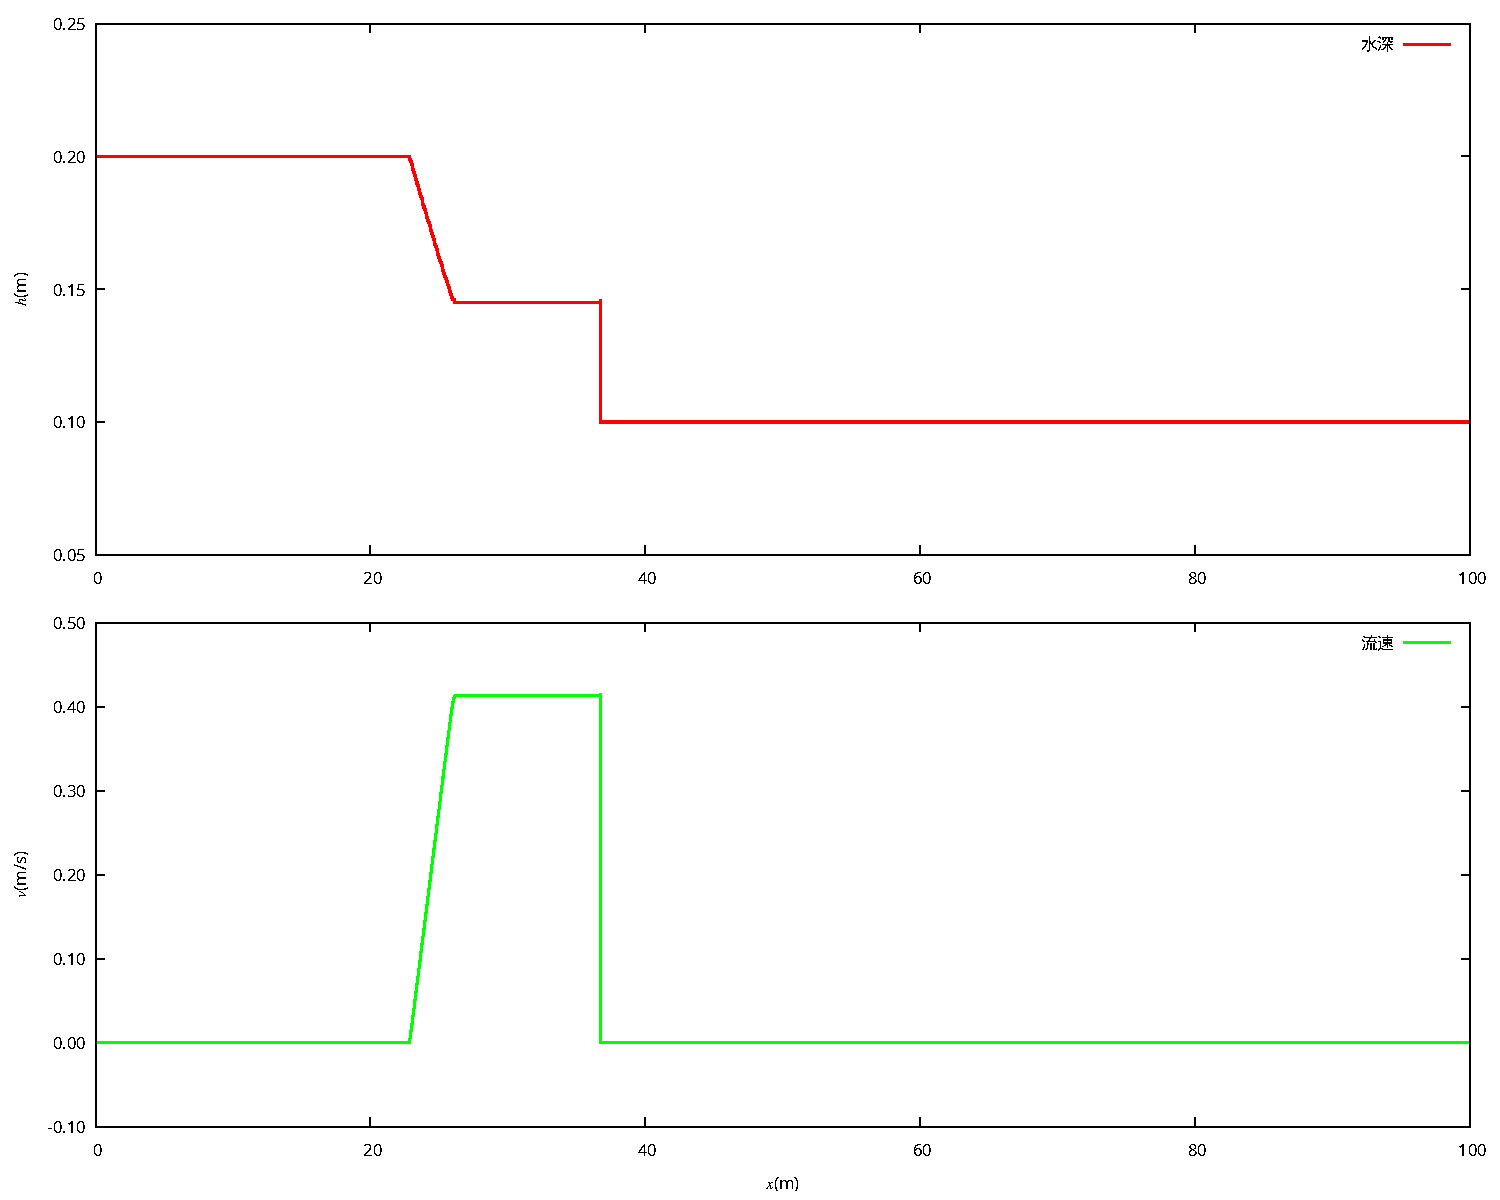
\includegraphics[width=8cm]{FgEx_tvd_result_t_5.pdf}
  \caption{MacCormack TVD格式计算结果}
  \label{FgEx_tvd_result_t_5}
\end{figure}



\section{二维泊松方程求解}
二维泊松方程是水力学中一种常见的方程,如速度势函数、流函数等,方程形式如下:
\begin{equation}
  \frac{\partial^{2} f}{\partial x^{2}} +
  \frac{\partial^{2} f}{\partial y^{2}}
  =
  S
\end{equation}
采用二阶偏导的二阶中心差分格式离散上式,可得
\begin{equation}
  \frac{f_{i+1,j} - 2f_{i, j} + f_{i-1,j}}{(\Delta x)^{2}} +
  \frac{f_{i,j+1} - 2f_{i, j} + f_{i,j-1}}{(\Delta y)^{2}} 
  =
  S_{i,j}
\end{equation}
对均匀网格,$\Delta x=\Delta y=h$,上式可写成
\begin{equation}
  f_{i+1, j} + f_{i-1,j } - 4f_{i,j} + f_{i, j+1} + f_{i, j-1} = h^{2}S_{i,j}
\end{equation}
求解上式可以用第4章的迭代解法。对雅克比迭代,上式的迭代式为
\begin{equation}
  f_{i, j}^{k+1} = 
\frac{1}{4}(f_{i-1,j }^{k} + f_{i, j-1}^{k} + f_{i+1, j}^{k} + f_{i, j+1}^{k}  - h^{2}S_{i,j})
\end{equation}
对高斯-赛德尔迭代,迭代式为
\begin{equation}
  f_{i, j}^{k+1} = 
\frac{1}{4}(f_{i-1,j }^{k+1} + f_{i, j-1}^{k+1} + f_{i+1, j}^{k} + f_{i, j+1}^{k}  - h^{2}S_{i,j})
\end{equation}
对超松弛迭代,迭代式为
\begin{equation}
  f_{i, j}^{k+1} = 
  (1-\alpha)f_{i, j}^{k}+
  \frac{\alpha}{4}(f_{i-1,j }^{k+1} + f_{i, j-1}^{k+1} + f_{i+1, j}^{k} + f_{i, j+1}^{k}  - h^{2}S_{i,j})
\end{equation}
松弛因子$\alpha$的取值范围为1\textasciitilde 2,一般取1.5。
\subsection{计算示例}
速度流函数满足
\begin{equation}
  \frac{\partial^{2}\psi }{\partial x^{2}} +
  \frac{\partial^{2}\psi }{\partial y^{2}} =
  0
\end{equation}
在一个长方形区域内,$0 \le x \le 75$,$0 \le y \le 50$。不透水地基多边形由下列点
形成(30,50)--(30,46) -- (31,46)
--(31,40) -- (32,40) -- (32,46) --(33,46) -- (33,48) -- (44,48) -- (44,46) --
(45,46) -- (45,50) -- (30,50)。 

在(0,50) -- (0,0) -- (75,0) -- (75,50)边界上流函
数$\psi=15$。
在(30,50)--(30,46)
--(31,40) -- (32,40) -- (32,46) --(33,46) -- (33,48) -- (44,48) -- (44,46) --
(45,46) -- (45,50)边界上$\psi=0$。
在(0,50)--(30,50),(45,50)--(75,50)这两条边界上$\frac{\partial\psi }{\partial n}
=0$。网格尺寸$\Delta x=\Delta y=0.5$。渗流计算区域和网格如图
\ref{fig_2dshenliu_region}所示。
\begin{figure}[htb]
  \centering
  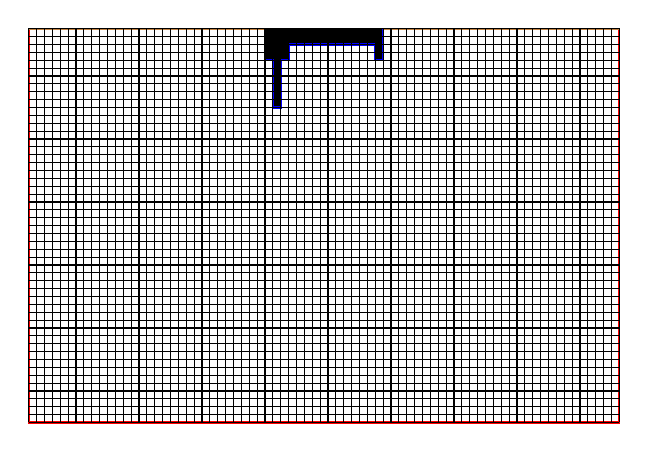
\begin{tikzpicture}
    \draw (0,5.0) -- (0,0) -- (7.5,0) -- (7.5,5.0) -- cycle;
    \draw[fill=black] (3.0,5.0)--(3.0,4.6) -- (3.1,4.6)
      --(3.1,4.0) -- (3.2,4.0) -- (3.2,4.6) --(3.3,4.6) -- (3.3,4.8) -- (4.4,4.8) --
      (4.4,4.6) --
      (4.5,4.6) -- (4.5,5.0) -- cycle; 
    \draw[red, thick] (0,5.0) -- (0,0) -- (7.5,0) -- (7.5,5.0);
    \draw[blue, thick] (3.0,5.0)--(3.0,4.6) -- (3.1,4.6)
      --(3.1,4.0) -- (3.2,4.0) -- (3.2,4.6) --(3.3,4.6) -- (3.3,4.8) -- (4.4,4.8) --
      (4.4,4.6) --
      (4.5,4.6) -- (4.5,5.0); 
    \draw[brown, thick] (0,5.0) -- (3.0,5.0);
    \draw[brown, thick] (4.5,5.0) -- (7.5,5.0);
    \foreach \y in {0,1,...,50}
    \draw[thin] (0, 0.1*\y) -- (7.5,0.1*\y);
    \foreach \x in {0,1,...,75}
    \draw[thin] (0.1*\x,0) -- (0.1*\x, 5.0);

  \end{tikzpicture}
  \caption{二维渗流流函数计算区域}
  \label{fig_2dshenliu_region}
\end{figure}

采用迭代法计算结果如图\ref{FgEx_2dshenliu_flood}和\ref{FgEx_2dshenliu_lines}所示。
不同迭代法的到达收敛所需迭代步数对比见图\ref{FgEx_2dshenliu_iteration}所示。
\begin{figure}[htb]
  \centering
  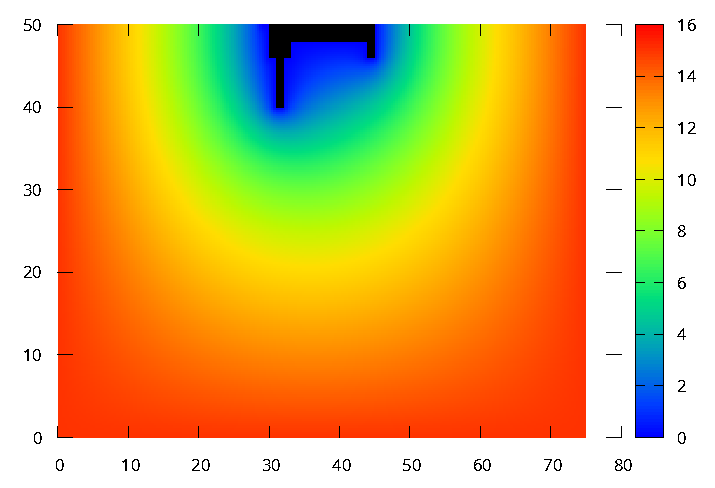
\includegraphics{FgEx_2dshenliu_flood.eps}
  \caption{二维渗流流函数分布云图}
  \label{FgEx_2dshenliu_flood}
\end{figure}
\begin{figure}[htb]
  \centering
  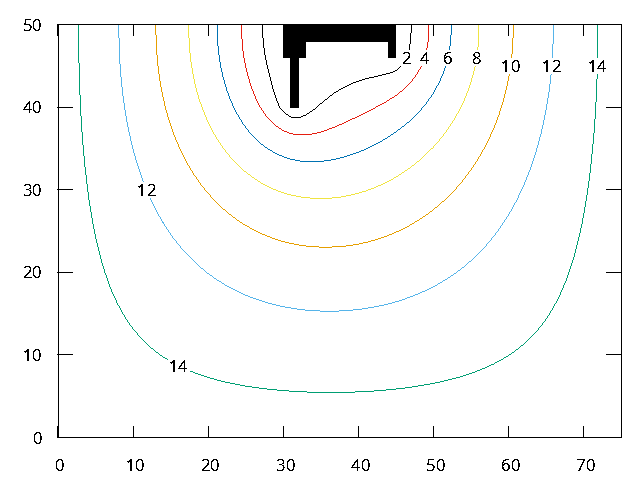
\includegraphics{FgEx_2dshenliu_lines.eps}
  \caption{二维渗流流函数等值线图}
  \label{FgEx_2dshenliu_lines}
\end{figure}
\begin{figure}[htb]
  \centering
  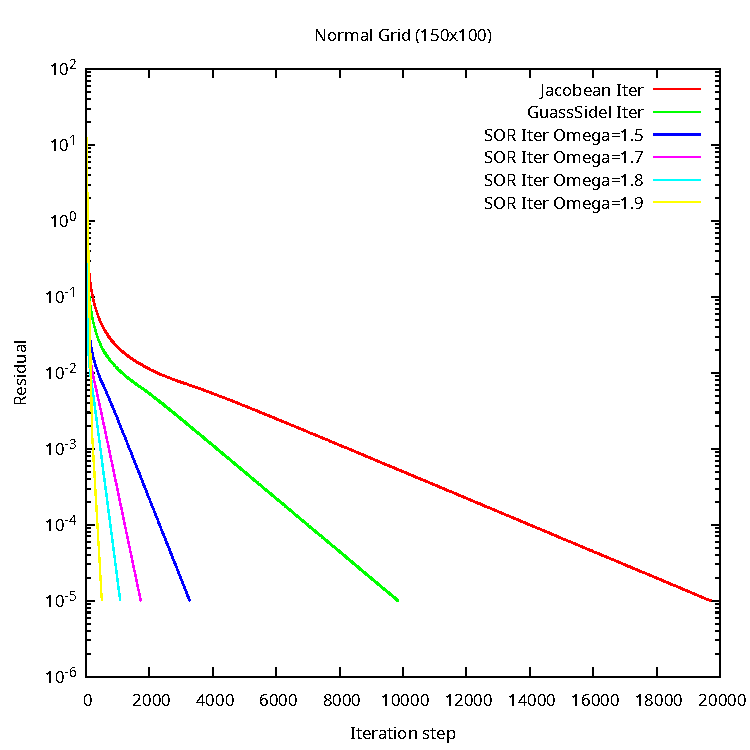
\includegraphics{FgEx_2dshenliu_iteration.pdf}
  \caption{不同迭代法收敛过程对比图}
  \label{FgEx_2dshenliu_iteration}
\end{figure}

%\section{二维方腔顶盖驱动流动求解}
%\subsection{问题描述}
%\subsection{SIMPLE算法求解}
%\subsection{涡量-流函数求解方法}

%\section{二维浅水方程求解}
%\subsection{网格基础}
%\subsection{求解算法}

